% Options for packages loaded elsewhere
\PassOptionsToPackage{unicode}{hyperref}
\PassOptionsToPackage{hyphens}{url}
%
\documentclass[
  english,
  man,floatsintext]{apa6}
\usepackage{amsmath,amssymb}
\usepackage{lmodern}
\usepackage{ifxetex,ifluatex}
\ifnum 0\ifxetex 1\fi\ifluatex 1\fi=0 % if pdftex
  \usepackage[T1]{fontenc}
  \usepackage[utf8]{inputenc}
  \usepackage{textcomp} % provide euro and other symbols
\else % if luatex or xetex
  \usepackage{unicode-math}
  \defaultfontfeatures{Scale=MatchLowercase}
  \defaultfontfeatures[\rmfamily]{Ligatures=TeX,Scale=1}
\fi
% Use upquote if available, for straight quotes in verbatim environments
\IfFileExists{upquote.sty}{\usepackage{upquote}}{}
\IfFileExists{microtype.sty}{% use microtype if available
  \usepackage[]{microtype}
  \UseMicrotypeSet[protrusion]{basicmath} % disable protrusion for tt fonts
}{}
\makeatletter
\@ifundefined{KOMAClassName}{% if non-KOMA class
  \IfFileExists{parskip.sty}{%
    \usepackage{parskip}
  }{% else
    \setlength{\parindent}{0pt}
    \setlength{\parskip}{6pt plus 2pt minus 1pt}}
}{% if KOMA class
  \KOMAoptions{parskip=half}}
\makeatother
\usepackage{xcolor}
\IfFileExists{xurl.sty}{\usepackage{xurl}}{} % add URL line breaks if available
\IfFileExists{bookmark.sty}{\usepackage{bookmark}}{\usepackage{hyperref}}
\hypersetup{
  pdftitle={Videogaming effects on mental health outcomes during three COVID-19 national lockdowns},
  pdfauthor={Sophie Hodgetts1, Glenn Patrick Williams1, \& Joe Butler1},
  pdflang={en-EN},
  pdfkeywords={keywords},
  hidelinks,
  pdfcreator={LaTeX via pandoc}}
\urlstyle{same} % disable monospaced font for URLs
\usepackage{graphicx}
\makeatletter
\def\maxwidth{\ifdim\Gin@nat@width>\linewidth\linewidth\else\Gin@nat@width\fi}
\def\maxheight{\ifdim\Gin@nat@height>\textheight\textheight\else\Gin@nat@height\fi}
\makeatother
% Scale images if necessary, so that they will not overflow the page
% margins by default, and it is still possible to overwrite the defaults
% using explicit options in \includegraphics[width, height, ...]{}
\setkeys{Gin}{width=\maxwidth,height=\maxheight,keepaspectratio}
% Set default figure placement to htbp
\makeatletter
\def\fps@figure{htbp}
\makeatother
\setlength{\emergencystretch}{3em} % prevent overfull lines
\providecommand{\tightlist}{%
  \setlength{\itemsep}{0pt}\setlength{\parskip}{0pt}}
\setcounter{secnumdepth}{-\maxdimen} % remove section numbering
% Make \paragraph and \subparagraph free-standing
\ifx\paragraph\undefined\else
  \let\oldparagraph\paragraph
  \renewcommand{\paragraph}[1]{\oldparagraph{#1}\mbox{}}
\fi
\ifx\subparagraph\undefined\else
  \let\oldsubparagraph\subparagraph
  \renewcommand{\subparagraph}[1]{\oldsubparagraph{#1}\mbox{}}
\fi
% Manuscript styling
\usepackage{upgreek}
\captionsetup{font=singlespacing,justification=justified}

% Table formatting
\usepackage{longtable}
\usepackage{lscape}
% \usepackage[counterclockwise]{rotating}   % Landscape page setup for large tables
\usepackage{multirow}		% Table styling
\usepackage{tabularx}		% Control Column width
\usepackage[flushleft]{threeparttable}	% Allows for three part tables with a specified notes section
\usepackage{threeparttablex}            % Lets threeparttable work with longtable

% Create new environments so endfloat can handle them
% \newenvironment{ltable}
%   {\begin{landscape}\begin{center}\begin{threeparttable}}
%   {\end{threeparttable}\end{center}\end{landscape}}
\newenvironment{lltable}{\begin{landscape}\begin{center}\begin{ThreePartTable}}{\end{ThreePartTable}\end{center}\end{landscape}}

% Enables adjusting longtable caption width to table width
% Solution found at http://golatex.de/longtable-mit-caption-so-breit-wie-die-tabelle-t15767.html
\makeatletter
\newcommand\LastLTentrywidth{1em}
\newlength\longtablewidth
\setlength{\longtablewidth}{1in}
\newcommand{\getlongtablewidth}{\begingroup \ifcsname LT@\roman{LT@tables}\endcsname \global\longtablewidth=0pt \renewcommand{\LT@entry}[2]{\global\advance\longtablewidth by ##2\relax\gdef\LastLTentrywidth{##2}}\@nameuse{LT@\roman{LT@tables}} \fi \endgroup}

% \setlength{\parindent}{0.5in}
% \setlength{\parskip}{0pt plus 0pt minus 0pt}

% \usepackage{etoolbox}
\makeatletter
\patchcmd{\HyOrg@maketitle}
  {\section{\normalfont\normalsize\abstractname}}
  {\section*{\normalfont\normalsize\abstractname}}
  {}{\typeout{Failed to patch abstract.}}
\patchcmd{\HyOrg@maketitle}
  {\section{\protect\normalfont{\@title}}}
  {\section*{\protect\normalfont{\@title}}}
  {}{\typeout{Failed to patch title.}}
\makeatother
\shorttitle{Covid Gaming}
\keywords{keywords\newline\indent Word count: X}
\usepackage{lineno}

\linenumbers
\usepackage{csquotes}
\usepackage{tipa}
\usepackage{float}
\usepackage{hyperref}
\usepackage{makecell}
\ifxetex
  % Load polyglossia as late as possible: uses bidi with RTL langages (e.g. Hebrew, Arabic)
  \usepackage{polyglossia}
  \setmainlanguage[]{english}
\else
  \usepackage[main=english]{babel}
% get rid of language-specific shorthands (see #6817):
\let\LanguageShortHands\languageshorthands
\def\languageshorthands#1{}
\fi
\ifluatex
  \usepackage{selnolig}  % disable illegal ligatures
\fi
\newlength{\cslhangindent}
\setlength{\cslhangindent}{1.5em}
\newlength{\csllabelwidth}
\setlength{\csllabelwidth}{3em}
\newenvironment{CSLReferences}[2] % #1 hanging-ident, #2 entry spacing
 {% don't indent paragraphs
  \setlength{\parindent}{0pt}
  % turn on hanging indent if param 1 is 1
  \ifodd #1 \everypar{\setlength{\hangindent}{\cslhangindent}}\ignorespaces\fi
  % set entry spacing
  \ifnum #2 > 0
  \setlength{\parskip}{#2\baselineskip}
  \fi
 }%
 {}
\usepackage{calc}
\newcommand{\CSLBlock}[1]{#1\hfill\break}
\newcommand{\CSLLeftMargin}[1]{\parbox[t]{\csllabelwidth}{#1}}
\newcommand{\CSLRightInline}[1]{\parbox[t]{\linewidth - \csllabelwidth}{#1}\break}
\newcommand{\CSLIndent}[1]{\hspace{\cslhangindent}#1}

\title{Videogaming effects on mental health outcomes during three COVID-19 national lockdowns}
\author{Sophie Hodgetts\textsuperscript{1}, Glenn Patrick Williams\textsuperscript{1}, \& Joe Butler\textsuperscript{1}}
\date{}


\authornote{

School of Psychology, Faculty of Health Sciences and Wellbeing, University of Sunderland, Sunderland, SR1 3SD, England, UK.

Pre-registration, data and code, and pre-print are available at\ldots{}

This preprint has not been peer reviewed.

The authors made the following contributions. Sophie Hodgetts: Conceptualisation, Investigation, Data Curation, Methodology, Project Administration, Resources, Writing - Original Draft Preparation, Writing - Review \& Editing; Glenn Patrick Williams: Conceptualization, Writing - Original Draft Preparation, Writing - Review \& Editing, Data Curation, Methodology, Formal Analysis, Visualization; Joe Butler: Conceptualization, Investigation, Methodology, Project Administration, Writing - Original Draft Preparation, Writing - Review \& Editing.

Correspondence concerning this article should be addressed to Sophie Hodgetts, Postal address. E-mail: \href{mailto:sophie.hodgetts@sunderland.ac.uk}{\nolinkurl{sophie.hodgetts@sunderland.ac.uk}}

}

\affiliation{\vspace{0.5cm}\textsuperscript{1} University of Sunderland}

\abstract{
Abstract goes here.
}



\begin{document}
\maketitle

\hypertarget{introduction}{%
\section{Introduction}\label{introduction}}

Intro here.

\hypertarget{study-1}{%
\section{Study 1}\label{study-1}}

\hypertarget{methods}{%
\subsection{Methods}\label{methods}}

\hypertarget{participants}{%
\subsubsection{Participants}\label{participants}}

Five hundred and seventy-one participants were recruited to take part in this study online via Qualtrics. Of which 344 provided full informed consent. One hundred and fifteen participants were excluded from this sample due to having completed less than 90\% of the questionnaire, providing invalid employment details (i.e.~stating they were both employed and unemployed) or for reporting having played no games before or during lockdown. A further 9 participants were removed from the analysis due to having more than 20\% of trials with missing data and/or having reported hours played more than 98 hours per week (i.e.~an average of 14 hours a day). From the remaining sample, only \texttt{data\_summary\$}01\_study-01\texttt{\$missing\_data\_counts\ \%\textgreater{}\%\ group\_by(is\_missing)\ \%\textgreater{}\%\ summarise(n\ =\ sum(n))\ \%\textgreater{}\%\ pivot\_wider(names\_from\ =\ is\_missing,\ values\_from\ =\ n)\ \%\textgreater{}\%\ mutate(percent\ =}TRUE\texttt{/}FALSE\texttt{)\ \%\textgreater{}\%\ pull(percent)}\% of trials had missing data, which was handled using multiple imputation with the mice R-package (van Buuren \& Groothuis-Oudshoorn, 2011).

After all exclusions we analysed data from 220 participants (age \emph{M} = 32.01, \emph{SD} = 8.96, Range = 19 - 72). On average participants took 25.77 minutes to complete the task (\emph{SD} = 91.26).

Figure~\ref{fig:study-one-situations-plot} shows the number of participants in a given employment situation during lockdown.

\begin{figure*}[!htbp]

{\centering \includegraphics[width=0.9\linewidth]{/Users/glennwilliams/Dropbox/GitHub/covid-gaming/03_plots/01_study-01/situation_combined} 

}

\caption{Count of participants by self-reported (a) employment status, (b) lockdown work situation, and (c) living situation.}\label{fig:study-one-situations-plot}
\end{figure*}

\hypertarget{procedure-and-materials}{%
\subsubsection{Procedure and Materials}\label{procedure-and-materials}}

\hypertarget{depression-anxiety-stress-scale-21-items-dass-21-antony-et-al.-1998-lovibond-lovibond-1995}{%
\paragraph{Depression, Anxiety, Stress Scale -- 21 items (DASS-21, Antony et al., 1998; Lovibond \& Lovibond, 1995)}\label{depression-anxiety-stress-scale-21-items-dass-21-antony-et-al.-1998-lovibond-lovibond-1995}}

The DASS-21 was used to measure mental health outcomes. This 21-item scale is comprised of three sub-scales: depression, anxiety, and stress. The analysis considered all three subscales individually. For each item, participants are required to indicate how often the item applies to them via a 4-point Likert scale (1 = Did not apply to me at all, 4 = Applied to me very much or most of the time).

\hypertarget{ucla-three-item-loneliness-scale-hughes-et-al.-2004}{%
\paragraph{UCLA Three-item Loneliness Scale (Hughes et al., 2004)}\label{ucla-three-item-loneliness-scale-hughes-et-al.-2004}}

The UCLA Three-item Loneliness Scale was used to measure of loneliness. The three items ask participants to indicate how often they felt that they lacked companionship, felt left out, and felt isolated from others, using a 3-point Likert scale (1 = Hardly ever, 3 = Often).

\hypertarget{video-gaming-habits-questionnaire-adapted-from-waris-et-al.-2019}{%
\paragraph{Video gaming habits questionnaire (adapted from Waris et al., 2019)}\label{video-gaming-habits-questionnaire-adapted-from-waris-et-al.-2019}}

To assess video gaming habits, we adapted the video gaming habits questionnaire as reported by Waris et al.~(2019). Participants were asked to indicate whether they played computer, console, or similar games, and to estimate how many hours they played on average per week. They were then asked to estimate, as percentages, how much time per week they spent playing the following game genres: card, mobile, action, first-person shooter, exercise/music/party, adventure/puzzle/role-playing, simulation, strategy, and brain training/education. For each genre, participants were also asked to indicate whether they played alone or with others.

\hypertarget{procedure}{%
\paragraph{Procedure}\label{procedure}}

After consenting, all participants completed a series of demographic questions (e.g., age, sex/gender, education/employment status, living arrangement). They were also asked to provide information regarding the effect lockdown had on their employment (e.g., furloughed, worked from home, continued as normal). All participants were then presented with the DASS-21, the Three-item Loneliness Scale, and the video gaming habits questionnaires. All questionnaires were administered twice during one survey session. In the first instance, participants were asked to complete the questionnaires with respect to how they felt four weeks before lockdown (i.e., February 2020). This allowed for an approximate baseline measure of each questionnaire. In the second instance, participants were asked to report how they currently felt (i.e., during lockdown).

\hypertarget{data-analysis-and-model-fitting}{%
\subsubsection{Data Analysis and Model Fitting}\label{data-analysis-and-model-fitting}}

We used R {[}Version 4.0.3; R Core Team (2020){]} and the R-packages \emph{BayesFactor} {[}Version 0.9.12.4.2; Morey and Rouder (2018){]}, \emph{bayestestR} {[}Version 0.9.0; Makowski, Ben-Shachar, and Lüdecke (2019){]}, \emph{brms} {[}Version 2.14.4; Bürkner (2017); Bürkner (2018){]}, \emph{here} {[}Version 1.0.1; Müller (2017){]}, \emph{mice} {[}Version 3.13.0; van Buuren and Groothuis-Oudshoorn (2011){]}, \emph{modelr} {[}Version 0.1.8; Wickham (2020){]}, \emph{papaja} {[}Version 0.1.0.9997; Aust and Barth (2020){]}, \emph{tidybayes} {[}Version 2.3.1; Kay (2020){]}, and \emph{tidyverse} {[}Version 1.3.0; Wickham et al. (2019){]} for all our analyses.

Prior to modelling the effect of lockdown and hours playing video games on mental health outcomes, we assessed whether gaming hours increased from baseline during lockdown. To do so, we used the \texttt{BayesFactor} R-package to perform a Bayesian paired-samples \emph{t}-test (with a default \(Cauchy(0, 0.707)\) prior) calculating the Bayes factor in support of the alternative hypothesis (i.e.~of a non-zero effect) in relation to the null hypothesis (i.e.~of a point-null effect) in regards to an increase in hours played after lockdown. Estimates of the posterior mean and 95\% credible intervals for the difference in hours played was obtained using Markov Chain Monte Carlo (MCMC) sampling with 1000 posterior samples.

Primary analyses aimed to estimate the effect of hours played in games before and after lockdown on mental health outcomes including depression, anxiety, and stress (as measured by the DAS21) and loneliness (as measured by the three-item loneliness scale). Given that all items are scored in each subscale of the DASS-21 and in the Three-item Loneliness Scale by summing responses to each item from a 1-7 Likert scale, the summed responses to these items are necessarily integers with a lower and upper bound and represent ordinal responses. To accommodate this, we analysed the data using ordinal models (Bürkner \& Vuorre, 2019). These models are more appropriate than those that assume the response variable is metric (e.g.~typical linear regression assuming data are drawn from a Gaussian distribution), which often result in poor effect size estimates (e.g.~predictions outside the possible range of values).

The models took the form of a cumulative linear model with a logit link function, assuming that the response variable is generated from categorisation of an unobserved continuous variable. These models were fitted using the \texttt{brm()} function from the brms R-package (Bürkner, 2018). These models contained a fixed effect of total hours played, lockdown period (i.e.~before or during lockdown), and the interaction between them. The categorical fixed effect of lockdown period was sum-coded (before = -1, after = 1) while the continuous fixed effect of total hours played was z-transformed. Thus, the intercept represents the grand mean and parameter estimates represent the impact of lockdown on mental health outcomes across the average hours played (i.e.~a main effect of lockdown period), the impact of hours played across the average of both time points (i.e.~a main effect of hours played), and their interaction. All models contained random intercepts per participant. Details of the priors for all models are outlined in the Appendix.

Parameter estimates and 95\% credible intervals were again obtained using MCMC sampling with 8000 posterior samples. We used the \texttt{hypothesis()} function from the brms R-package to calculate Bayes factors using the Savage-Dickey density ratio to evaluate evidence in support of the null hypothesis for each parameter estimate (i.e.~for a point-null effect of 0) in relation to the alternative hypothesis (i.e.~of a non-zero effect). The Supplemental Material contains prior-predictive and posterior-predictive checks along with sensitivity checks evaluating how the prior scale affects parameter estimates and Bayes factors.

Additional analyses were used to further delineate any effects of gaming habits on changes to mental health outcomes. Change scores for mental health outcomes were calculated subtracting scores during lockdown from before lockdown) and the effect of total hours played during lockdown was estimated on this outcome as a fixed effect. Here, simple Bayesian linear models were used to model change scores (i.e.~assuming the data were drawn from a Gaussian distribution). Finally, models were fitted evaluating whether depression, anxiety, or stress during lockdown are affected by any difference in hours played before and during lockdown, and further whether this effect is moderated by loneliness during lockdown. These models contained fixed effects of difference scores for hours played before and during lockdown, loneliness during lockdown, and their interaction. Again, these models took the form of a cumulative linear model with a logit link function, with continuous fixed effects of the difference in hours played and loneliness during lockdown. Parameter estimates and hypothesis tests were carried out for these models using the same methods outlined above. Similarly, priors for these models are outlined in the Appendix and model checks are reported in the Supplemental Material.

\hypertarget{results}{%
\subsection{Results}\label{results}}

The average mental health outcomes and total hours played before and during lockdown are depicted in Figure~\ref{fig:study-one-mh-raincloud-plot}.

\begin{figure*}[!htbp]

{\centering \includegraphics[width=0.9\linewidth]{/Users/glennwilliams/Dropbox/GitHub/covid-gaming/03_plots/01_study-01/mh_raincloud} 

}

\caption{Mental health outcomes for the depression, anxiety, stress, and loneliness along with total hours played before and during lockdown. Dots represent individual participants' mean (jittered) scores.}\label{fig:study-one-mh-raincloud-plot}
\end{figure*}

We found evidence in support of the alternative model (i.e.~of a difference in means) when compared to the point null hypothesis, \(BF_{10}\) \textgreater{} 1,000,000 (± 0.00\%), with posterior summaries showing an average increase in total hours played of 9.84 (\emph{SD} = 1.20, 95\% CI = {[}7.44, 12.25{]}). Having confirmed a general increase in hours spent gaming after lockdown we next established the role of total hours spent gaming on mental health outcomes.

Figure~\ref{fig:study-one-mh-main-predictions-plot} shows posterior estimates for mental health outcomes before and during lockdown as a function of the total hours played before or during lockdown.

\begin{figure*}[!htbp]

{\centering \includegraphics[width=0.9\linewidth]{/Users/glennwilliams/Dropbox/GitHub/covid-gaming/03_plots/01_study-01/01_main-plots/mh_main_predictions} 

}

\caption{Mental health outcomes for the depression, anxiety, stress, and loneliness measures as a function of total hours played before and during lockdown. Lines and ribbons indicate the posterior median ± 95\% credible intervals.}\label{fig:study-one-mh-main-predictions-plot}
\end{figure*}

Table~\ref{tab:study-one-mh-bayes-pre-post} shows the population-level parameter estimates, their standard error, and 95\% credible intervals on the log scale, along with Bayes factors in support of the null hypothesis relative to the alternative hypothesis for both main effects and their interaction for each model.

\begin{table}[!htbp]

\begin{center}
\begin{threeparttable}

\caption{\label{tab:study-one-mh-bayes-pre-post}Parameter estimates, 95\% credible intervals, and Bayes factors evaluating evidence in support of the point null hypothesis that each parameter estimate is equal to zero for the effect of lockdown period, total hours played, and their interaction on mental health outcomes.}

\begin{tabular}{lllll}
\toprule
Parameter & \multicolumn{1}{c}{$Est.$} & \multicolumn{1}{c}{$SE$} & \multicolumn{1}{c}{95\% CI} & \multicolumn{1}{c}{$BF_{01}$}\\
\midrule
Depression &  &  &  & \\
\ \ \ Lockdown Period & 0.45 & 0.10 & {}[0.26, 0.64] & < .001\\
\ \ \ Total Hours & 0.36 & 0.17 & {}[0.02, 0.70] & 0.71\\
\ \ \ Lockdown Period by Hours & -0.07 & 0.11 & {}[-0.28, 0.14] & 7.48\\
Anxiety &  &  &  & \\
\ \ \ Lockdown Period & 0.19 & 0.10 & {}[-0.00, 0.39] & 1.59\\
\ \ \ Total Hours & 0.33 & 0.17 & {}[0.00, 0.68] & 0.94\\
\ \ \ Lockdown Period by Hours & -0.08 & 0.11 & {}[-0.29, 0.13] & 6.92\\
Stress &  &  &  & \\
\ \ \ Lockdown Period & 0.39 & 0.10 & {}[0.20, 0.58] & < .001\\
\ \ \ Total Hours & 0.12 & 0.16 & {}[-0.19, 0.42] & 5.02\\
\ \ \ Lockdown Period by Hours & 0.05 & 0.10 & {}[-0.15, 0.26] & 9.15\\
Loneliness &  &  &  & \\
\ \ \ Lockdown Period & 0.62 & 0.11 & {}[0.41, 0.83] & < .001\\
\ \ \ Total Hours & 0.01 & 0.17 & {}[-0.33, 0.34] & 5.86\\
\ \ \ Lockdown Period by Hours & 0.07 & 0.11 & {}[-0.15, 0.30] & 7.35\\
\bottomrule
\addlinespace
\end{tabular}

\begin{tablenotes}[para]
\normalsize{\textit{Note.} Higher Bayes factor values indicate support for the null hypothesis while lower numbers indicate support for the alternative hypothesis (i.e. of a non-null effect). Effects are reported on the log scale.}
\end{tablenotes}

\end{threeparttable}
\end{center}

\end{table}

Table~\ref{tab:study-one-mh-bayes-pre-post} shows evidence in support of the alternative hypothesis for the effect of lockdown period on depression, stress, and loneliness measures whereby parameter estimates show a reliable increase in these measures during lockdown. While a similar trend is shown for anxiety, the parameter estimate is small, with the credible intervals spanning 0, and with an inconclusive Bayes factor. There is reliable evidence in support of the null hypothesis that total hours played has no effect on loneliness or stress across both lockdown periods. However, while there is evidence that as hours played increases depression and anxiety also increase these effects span a range of negligible to rather large effects and similarly have inconclusive Bayes factors. For all mental health outcomes the lockdown period does not interact with any effect of total hours played.

Table~\ref{tab:study-one-mh-bayes-l-diff} shows the population-level parameter estimates, their standard error, and 95\% credible intervals for the effect of hours played during lockdown on changes to mental health outcomes.

\begin{table}[!htbp]

\begin{center}
\begin{threeparttable}

\caption{\label{tab:study-one-mh-bayes-l-diff}Parameter estimates, 95\% credible intervals, and Bayes factors evaluating evidence in support of the point null hypothesis that hours played during lockdown has no impact on changes to mental health outcomes.}

\begin{tabular}{lllll}
\toprule
Model & \multicolumn{1}{c}{$Est.$} & \multicolumn{1}{c}{$SE$} & \multicolumn{1}{c}{95\% CI} & \multicolumn{1}{c}{$BF_{01}$}\\
\midrule
Depression & 0.00 & 0.03 & {}[-0.06, 0.05] & 18.98\\
Anxiety & 0.00 & 0.02 & {}[-0.03, 0.03] & 32.24\\
Stress & 0.01 & 0.02 & {}[-0.03, 0.06] & 19.08\\
Loneliness & 0.00 & 0.00 & {}[-0.01, 0.01] & 80.60\\
\bottomrule
\addlinespace
\end{tabular}

\begin{tablenotes}[para]
\normalsize{\textit{Note.} Higher Bayes factor values indicate support for the null hypothesis while lower numbers indicate support for the alternative hypothesis (i.e. of a non-null effect). Effects are reported on the log scale.}
\end{tablenotes}

\end{threeparttable}
\end{center}

\end{table}

Table~\ref{tab:study-one-mh-bayes-l-diff} shows evidence in support of the null hypothesis of no impact of hours played during lockdown on changes to all mental health outcomes.

We next tested whether any effect of changes to hours played on mental health outcomes during lockdown is moderated by loneliness during lockdown. Figure~\ref{fig:study-one-moderation-predictions-plot} shows posterior predictions for mental health outcomes during lockdown as a function of difference in hours played with lines fitted to the average loneliness scores during lockdown ± 1 \emph{SD} of the mean.

\begin{figure*}[!htbp]

{\centering \includegraphics[width=0.9\linewidth]{/Users/glennwilliams/Dropbox/GitHub/covid-gaming/03_plots/01_study-01/01_main-plots/moderation_plots} 

}

\caption{Mental health outcomes for the depression, anxiety, and stress measures as a function of the difference in hours played before and during lockdown and loneliness scores during lockdown. Lines and ribbons indicate the posterior mean ± 95\% credible intervals, with each line representing the mean loneliness score ± 1 SD.}\label{fig:study-one-moderation-predictions-plot}
\end{figure*}

Table~\ref{tab:study-one-mh-moderation} shows the population-level parameter estimates, their standard error, and 95\% credible intervals on the log scale, along with Bayes factors in support of the null hypothesis relative to the alternative hypothesis for both main effects and their interaction for each model.

\begin{table}[!htbp]

\begin{center}
\begin{threeparttable}

\caption{\label{tab:study-one-mh-moderation}Parameter estimates, 95\% credible intervals, and Bayes factors evaluating evidence in support of the point null hypothesis that each parameter estimate is equal to zero for the effect of difference in hours played, loneliness during lockdown, and their interaction on mental health outcomes.}

\begin{tabular}{lllll}
\toprule
Parameter & \multicolumn{1}{c}{$Est.$} & \multicolumn{1}{c}{$SE$} & \multicolumn{1}{c}{95\% CI} & \multicolumn{1}{c}{$BF_{01}$}\\
\midrule
Depression &  &  &  & \\
\ \ \ Difference in Hours Played & 0.01 & 0.02 & {}[-0.03, 0.06] & 39.41\\
\ \ \ Loneliness During Lockdown & 0.70 & 0.08 & {}[0.55, 0.85] & < .001\\
\ \ \ Hours by Loneliness & 0.00 & 0.00 & {}[-0.01, 0.01] & 256.99\\
Anxiety &  &  &  & \\
\ \ \ Difference in Hours Played & 0.03 & 0.02 & {}[-0.01, 0.07] & 19.10\\
\ \ \ Loneliness During Lockdown & 0.40 & 0.08 & {}[0.25, 0.55] & < .001\\
\ \ \ Hours by Loneliness & 0.00 & 0.00 & {}[-0.01, 0.00] & 197.66\\
Stress &  &  &  & \\
\ \ \ Difference in Hours Played & 0.03 & 0.02 & {}[-0.02, 0.07] & 22.60\\
\ \ \ Loneliness During Lockdown & 0.53 & 0.08 & {}[0.38, 0.68] & < .001\\
\ \ \ Hours by Loneliness & 0.00 & 0.00 & {}[-0.01, 0.00] & 224.12\\
\bottomrule
\addlinespace
\end{tabular}

\begin{tablenotes}[para]
\normalsize{\textit{Note.} Higher Bayes factor values indicate support for the null hypothesis while lower numbers indicate support for the alternative hypothesis (i.e. of a non-null effect). Effects are reported on the log scale.}
\end{tablenotes}

\end{threeparttable}
\end{center}

\end{table}

Table~\ref{tab:study-one-mh-moderation} shows evidence in support of the null hypothesis for any effect of difference in hours played or any moderating effect of loneliness on hours played for all mental health outcomes. Here, all parameter estimates are very small, with credible intervals spanning zero and with Bayes factors in support of the null hypothesis. relative to the alternative hypothesis. However, there is substantial evidence in support of higher scores for loneliness during lockdown leading to poorer mental health outcomes during lockdown. Here, effects are positive and large, with Bayes factors in support of the alternative hypothesis relative to the null hypothesis.

\hypertarget{interim-summary}{%
\subsection{Interim Summary}\label{interim-summary}}

Study 1 showed that while on average participants played video games for more hours during lockdown than before lockdown, the hours played or changes to hours played gaming largely have no effect on mental health outcomes. However, mental health outcomes were worse during lockdown when compared to before lockdown. There was no effect of the difference in hours playing games on mental health outcomes, nor any moderating effect of loneliness on the difference in hours playing games. Rather, we show that as loneliness during lockdown increases, stress, anxiety, and depression also increase.

\hypertarget{study-2}{%
\section{Study 2}\label{study-2}}

The mediation analysis in Study 1 revealed that loneliness did not moderate the relationship between video gaming and DASS-21 scores. However, the Three-Item Loneliness Scale used in Study 1 was not necessarily the optimal measure for the required analysis. Specifically, this measure is designed to provide binary classifications of ``lonely'' and ``not lonely,'' as opposed to an average loneliness score (Steptoe et al., 2013). Moreover, the scale measures loneliness as a unitary concept, rather than multidimensional constructure comprised of different forms of loneliness (Weiss, 1973). Therefore, to increase the validity and sensitivity of the loneliness measurement, Study 2 included the De Jong-Gierveld 11-Item Loneliness Scale (de Jong-Gierveld \& Kamphuls, 1985). This scale provides measurements of both emotional and social loneliness and may therefore be more appropriate for assessing the specific forms of loneliness experienced during lockdown.

\hypertarget{methods-1}{%
\subsection{Methods}\label{methods-1}}

\hypertarget{participants-1}{%
\subsubsection{Participants}\label{participants-1}}

Two hundred and ten participants were recruited to take part in this study online via Qualtrics. Of which 158 provided full informed consent. Sixty-two participants were excluded from this sample due to having completed less than 90\% of the questionnaire, providing invalid employment details (i.e.~stating they were both employed and unemployed) or for reporting having played no games before or during lockdown. A further 20 participants were removed from the analysis due to having more than 20\% of trials with missing data and/or having reported hours played more than 98 hours per week (i.e.~an average of 14 hours a day). From the remaining sample, only no trials had missing data.

After all exclusions we analysed data from 76 participants (age \emph{M} = 29.96, \emph{SD} = 8.24, Range = 19 - 64). On average participants took 17.00 minutes to complete the task (\emph{SD} = 15.36).

Figure~\ref{fig:study-two-situations-plot} shows the number of participants in a given employment situation during lockdown.

\begin{figure*}[!htbp]

{\centering \includegraphics[width=0.9\linewidth]{/Users/glennwilliams/Dropbox/GitHub/covid-gaming/03_plots/02_study-02/situation_combined} 

}

\caption{Count of participants by self-reported (a) employment status, (b) lockdown work situation, and (c) living situation.}\label{fig:study-two-situations-plot}
\end{figure*}

\hypertarget{procedure-and-materials-1}{%
\subsubsection{Procedure and Materials}\label{procedure-and-materials-1}}

The DASS-21 and UCLA Three-Item Loneliness scales were presented identically to Study 1. The assessment of video gaming habits was presented using sliding scales as opposed to requiring participants to manually type in their responses.

\hypertarget{the-de-jong-gierveld-11-item-loneliness-scale-de-jong-gierveld-kamphuls-1985.}{%
\paragraph{The De Jong-Gierveld 11-Item Loneliness Scale (de Jong-Gierveld \& Kamphuls, 1985).}\label{the-de-jong-gierveld-11-item-loneliness-scale-de-jong-gierveld-kamphuls-1985.}}

This scale was used in addition to the UCLA scale to measure loneliness. The 11 items ask participants to respond ``yes,'' ``no,'' or ``more or less'' to a series of statements regarding either emotional (e.g., ``I experience a general sense of emptiness.'') or social (e.g., ``There are enough people I feel close to.'') loneliness.

\hypertarget{procedure-1}{%
\paragraph{Procedure}\label{procedure-1}}

All questionnaire procedures were identical to Study 1, with wording updated to the lockdown under investigation (i.e.~before/during November 2020).

\hypertarget{results-1}{%
\subsection{Results}\label{results-1}}

The average mental health outcomes and total hours played before and during lockdown are depicted in Figure~\ref{fig:study-two-mh-raincloud-plot}.

\begin{figure*}[!htbp]

{\centering \includegraphics[width=0.9\linewidth]{/Users/glennwilliams/Dropbox/GitHub/covid-gaming/03_plots/02_study-02/mh_raincloud} 

}

\caption{Mental health outcomes for the depression, anxiety, stress, and loneliness along with total hours played before and during lockdown. Dots represent individual participants' mean (jittered) scores.}\label{fig:study-two-mh-raincloud-plot}
\end{figure*}

We found support of the null model (i.e.~the point null hypothesis) compared to the alternative model (i.e.~of a difference in means), \(BF_{01}\) = 7.70 (± 0.00\%), with posterior summaries showing an average increase in total hours played of 0.66 (\emph{SD} = 2.62, 95\% CI = {[}-4.65, 5.68{]}). Despite showing no change in hours spent gaming, we applied the same models to the second lockdown as in Study 1.

Figure~\ref{fig:study-two-mh-main-predictions-plot} shows posterior estimates for mental health outcomes before and during lockdown as a function of the total hours played before or during lockdown.

\begin{figure*}[!htbp]

{\centering \includegraphics[width=0.9\linewidth]{/Users/glennwilliams/Dropbox/GitHub/covid-gaming/03_plots/02_study-02/01_main-plots/mh_main_predictions} 

}

\caption{Mental health outcomes for the depression, anxiety, stress, and loneliness measures as a function of total hours played before and during lockdown. Lines and ribbons indicate the posterior median ± 95\% credible intervals.}\label{fig:study-two-mh-main-predictions-plot}
\end{figure*}

Table~\ref{tab:study-two-mh-bayes-pre-post} shows the population-level parameter estimates, their standard error, and 95\% credible intervals on the log scale, along with Bayes factors in support of the null hypothesis relative to the alternative hypothesis for both main effects and their interaction for each model.

\begin{table}[!htbp]

\begin{center}
\begin{threeparttable}

\caption{\label{tab:study-two-mh-bayes-pre-post}Parameter estimates, 95\% credible intervals, and Bayes factors evaluating evidence in support of the point null hypothesis that each parameter estimate is equal to zero for the effect of lockdown period, total hours played, and their interaction on mental health outcomes.}

\begin{tabular}{lllll}
\toprule
Parameter & \multicolumn{1}{c}{$Est.$} & \multicolumn{1}{c}{$SE$} & \multicolumn{1}{c}{95\% CI} & \multicolumn{1}{c}{$BF_{01}$}\\
\midrule
Depression &  &  &  & \\
\ \ \ Lockdown Period & 0.18 & 0.15 & {}[-0.11, 0.46] & 3.42\\
\ \ \ Total Hours & 0.80 & 0.27 & {}[0.29, 1.33] & 0.02\\
\ \ \ Lockdown Period by Hours & 0.00 & 0.17 & {}[-0.32, 0.33] & 5.92\\
Anxiety &  &  &  & \\
\ \ \ Lockdown Period & 0.07 & 0.15 & {}[-0.22, 0.37] & 6.01\\
\ \ \ Total Hours & 0.60 & 0.26 & {}[0.10, 1.10] & 0.25\\
\ \ \ Lockdown Period by Hours & 0.18 & 0.16 & {}[-0.15, 0.50] & 3.70\\
Stress &  &  &  & \\
\ \ \ Lockdown Period & -0.07 & 0.14 & {}[-0.34, 0.21] & 6.13\\
\ \ \ Total Hours & 0.63 & 0.26 & {}[0.12, 1.15] & 0.20\\
\ \ \ Lockdown Period by Hours & 0.25 & 0.17 & {}[-0.07, 0.58] & 1.87\\
Loneliness &  &  &  & \\
\ \ \ Lockdown Period & 0.14 & 0.15 & {}[-0.16, 0.44] & 4.26\\
\ \ \ Total Hours & 0.21 & 0.26 & {}[-0.30, 0.72] & 2.77\\
\ \ \ Lockdown Period by Hours & 0.01 & 0.17 & {}[-0.33, 0.34] & 5.89\\
\bottomrule
\addlinespace
\end{tabular}

\begin{tablenotes}[para]
\normalsize{\textit{Note.} Higher Bayes factor values indicate support for the null hypothesis while lower numbers indicate support for the alternative hypothesis (i.e. of a non-null effect). Effects are reported on the log scale.}
\end{tablenotes}

\end{threeparttable}
\end{center}

\end{table}

Table~\ref{tab:study-two-mh-bayes-pre-post} shows evidence in support of the null hypothesis relative to the alternative hypothesis for the effect of lockdown period on all mental health outcomes. However, there is evidence in support of the alternative hypothesis relative to the null hypothesis with regard to total hours played for depression, anxiety, and stress. Here, higher total hours played is associated with poorer mental health outcomes across both lockdown periods. For loneliness the effect of total hours played is small, with the credible interval spanning zero and with evidence in support of the null hypothesis relative to the alternative hypothesis. For all mental health outcomes the lockdown period does not interact with any effect of total hours played.

Table~\ref{tab:study-two-mh-bayes-l-diff} shows the population-level parameter estimates, their standard error, and 95\% credible intervals for the effect of hours played during lockdown on changes to mental health outcomes.

\begin{table}[!htbp]

\begin{center}
\begin{threeparttable}

\caption{\label{tab:study-two-mh-bayes-l-diff}Parameter estimates, 95\% credible intervals, and Bayes factors evaluating evidence in support of the point null hypothesis that hours played during lockdown has no impact on changes to mental health outcomes.}

\begin{tabular}{lllll}
\toprule
Model & \multicolumn{1}{c}{$Est.$} & \multicolumn{1}{c}{$SE$} & \multicolumn{1}{c}{95\% CI} & \multicolumn{1}{c}{$BF_{01}$}\\
\midrule
Depression & 0.04 & 0.03 & {}[-0.03, 0.10] & 7.22\\
Anxiety & 0.05 & 0.02 & {}[0.00, 0.09] & 3.41\\
Stress & 0.07 & 0.03 & {}[0.02, 0.13] & 0.58\\
Loneliness & 0.00 & 0.01 & {}[-0.02, 0.02] & 58.51\\
\bottomrule
\addlinespace
\end{tabular}

\begin{tablenotes}[para]
\normalsize{\textit{Note.} Higher Bayes factor values indicate support for the null hypothesis while lower numbers indicate support for the alternative hypothesis (i.e. of a non-null effect). Effects are reported on the log scale.}
\end{tablenotes}

\end{threeparttable}
\end{center}

\end{table}

Table~\ref{tab:study-two-mh-bayes-l-diff} shows evidence in support of the null hypothesis of no impact of hours played during lockdown on changes to depression, anxiety, and loneliness. For changes to anxiety the parameter estimate is small, with the credible interval showing a range of values from nearly 0 to a small upper limit, and with an inconclusive Bayes factor.

We next tested whether any effect of changes to hours played on mental health outcomes during lockdown is moderated by loneliness during lockdown. Figure~\ref{fig:study-two-moderation-predictions-plot} shows posterior predictions for mental health outcomes during lockdown as a function of difference in hours played with lines fitted to the average loneliness scores during lockdown ± 1 \emph{SD} of the mean.

\begin{figure*}[!htbp]

{\centering \includegraphics[width=0.9\linewidth]{/Users/glennwilliams/Dropbox/GitHub/covid-gaming/03_plots/02_study-02/01_main-plots/moderation_plots} 

}

\caption{Mental health outcomes for the depression, anxiety, and stress measures as a function of the difference in hours played before and during lockdown and loneliness scores during lockdown. Lines and ribbons indicate the posterior mean ± 95\% credible intervals, with each line representing the mean loneliness score ± 1 SD.}\label{fig:study-two-moderation-predictions-plot}
\end{figure*}

Table~\ref{tab:study-two-mh-moderation} shows the population-level parameter estimates, their standard error, and 95\% credible intervals on the log scale, along with Bayes factors in support of the null hypothesis relative to the alternative hypothesis for both main effects and their interaction for each model.

\begin{table}[!htbp]

\begin{center}
\begin{threeparttable}

\caption{\label{tab:study-two-mh-moderation}Parameter estimates, 95\% credible intervals, and Bayes factors evaluating evidence in support of the point null hypothesis that each parameter estimate is equal to zero for the effect of difference in hours played, loneliness during lockdown, and their interaction on mental health outcomes.}

\begin{tabular}{lllll}
\toprule
Parameter & \multicolumn{1}{c}{$Est.$} & \multicolumn{1}{c}{$SE$} & \multicolumn{1}{c}{95\% CI} & \multicolumn{1}{c}{$BF_{01}$}\\
\midrule
Depression &  &  &  & \\
\ \ \ Difference in Hours Played & -0.01 & 0.03 & {}[-0.06, 0.04] & 35.55\\
\ \ \ Loneliness During Lockdown & 0.35 & 0.07 & {}[0.22, 0.49] & < .001\\
\ \ \ Hours by Loneliness & 0.00 & 0.00 & {}[-0.00, 0.01] & 233.20\\
Anxiety &  &  &  & \\
\ \ \ Difference in Hours Played & 0.02 & 0.03 & {}[-0.03, 0.07] & 32.25\\
\ \ \ Loneliness During Lockdown & 0.22 & 0.06 & {}[0.10, 0.35] & 0.05\\
\ \ \ Hours by Loneliness & 0.00 & 0.00 & {}[-0.01, 0.01] & 303.03\\
Stress &  &  &  & \\
\ \ \ Difference in Hours Played & 0.05 & 0.03 & {}[0.00, 0.10] & 6.11\\
\ \ \ Loneliness During Lockdown & 0.21 & 0.07 & {}[0.08, 0.34] & 0.08\\
\ \ \ Hours by Loneliness & 0.00 & 0.00 & {}[-0.01, 0.00] & 129.74\\
\bottomrule
\addlinespace
\end{tabular}

\begin{tablenotes}[para]
\normalsize{\textit{Note.} Higher Bayes factor values indicate support for the null hypothesis while lower numbers indicate support for the alternative hypothesis (i.e. of a non-null effect). Effects are reported on the log scale.}
\end{tablenotes}

\end{threeparttable}
\end{center}

\end{table}

Table~\ref{tab:study-two-mh-moderation} shows evidence in support of the null hypothesis for any effect of difference in hours played or any moderating effect of loneliness on hours played for all mental health outcomes. Here, all parameter estimates are very small, with credible intervals spanning zero and with Bayes factors in support of the null hypothesis relative to the alternative hypothesis. However, there is substantial evidence in support of higher scores for loneliness during lockdown leading to poorer mental health outcomes during lockdown. Here, effects are positive and large, with Bayes factors in support of the alternative hypothesis relative to the null hypothesis.

\hypertarget{interim-summary-1}{%
\subsection{Interim Summary}\label{interim-summary-1}}

Unlike Study 1, Study 2 showed no average increase in hours spent gaming during lockdown when compared to before lockdown. In contrast to Study 1, there was no overall impact of lockdown period on mental health outcomes, but instead as hours spent gaming increased there were more negative outcomes for depression, anxiety, and stress, regardless of lockdown period. Additionally, while more hours spent gaming during lockdown was associated with a greater increase in anxiety, as in Study 1 hours spent gaming during lockdown had no effect on depression, anxiety, and stress. Replicating effects for Study 1, we found that higher scores for loneliness during lockdown led to poorer mental health outcomes during lockdown. Again, there was no effect of the the difference in hours playing games on mental health outcomes, nor any moderating effect of loneliness on the difference in hours playing games.

\hypertarget{study-3}{%
\section{Study 3}\label{study-3}}

{[}justification needed here -- might be easier once we have the results plugged in above?{]}

\hypertarget{methods-2}{%
\subsection{Methods}\label{methods-2}}

\hypertarget{participants-2}{%
\subsubsection{Participants}\label{participants-2}}

One hundred and five participants were recruited to take part in this study online via Qualtrics. Of which 86 provided full informed consent. Twenty-six participants were excluded from this sample due to having completed less than 90\% of the questionnaire, providing invalid employment details (i.e.~stating they were both employed and unemployed) or for reporting having played no games before or during lockdown. A further 5 participants were removed from the analysis due to having more than 20\% of trials with missing data and/or having reported hours played more than 98 hours per week (i.e.~an average of 14 hours a day). From the remaining sample, no trials had missing data.

After all exclusions we analysed data from 55 participants (age \emph{M} = 30.49, \emph{SD} = 7.65, Range = 19 - 51). On average participants took 116.57 minutes to complete the task (\emph{SD} = 737.51).

Figure~\ref{fig:study-three-situations-plot} shows the number of participants in a given employment situation during lockdown.

\begin{figure*}[!htbp]

{\centering \includegraphics[width=0.9\linewidth]{/Users/glennwilliams/Dropbox/GitHub/covid-gaming/03_plots/03_study-03/situation_combined} 

}

\caption{Count of participants by self-reported (a) employment status, (b) lockdown work situation, and (c) living situation.}\label{fig:study-three-situations-plot}
\end{figure*}

\hypertarget{procedure-and-materials-2}{%
\subsubsection{Procedure and Materials}\label{procedure-and-materials-2}}

All questionnaire procedures were identical to Study 2, with wording updated to the lockdown under investigation (i.e., since the beginning of January 2021).

\hypertarget{results-2}{%
\subsection{Results}\label{results-2}}

The average mental health outcomes and total hours played before and during lockdown are depicted in Figure~\ref{fig:study-three-mh-raincloud-plot}.

\begin{figure*}[!htbp]

{\centering \includegraphics[width=0.9\linewidth]{/Users/glennwilliams/Dropbox/GitHub/covid-gaming/03_plots/03_study-03/mh_raincloud} 

}

\caption{Mental health outcomes for the depression, anxiety, stress, and loneliness along with total hours played before and during lockdown. Dots represent individual participants' mean (jittered) scores.}\label{fig:study-three-mh-raincloud-plot}
\end{figure*}

We show inconclusive evidence in support of the alternative model (i.e.~of a difference in means) relative to the null model (i.e.~the point null hypothesis), \(BF_{10}\) = 1.52 (± 0.00\%), with posterior summaries showing an average increase in total hours played of 5.17 (\emph{SD} = 2.37, 95\% CI = {[}0.60, 9.63{]}). Regardless, we applied the same models to the second lockdown as in Study 1.

Figure~\ref{fig:study-three-mh-main-predictions-plot} shows posterior estimates for mental health outcomes before and during lockdown as a function of the total hours played before or during lockdown.

\begin{figure*}[!htbp]

{\centering \includegraphics[width=0.9\linewidth]{/Users/glennwilliams/Dropbox/GitHub/covid-gaming/03_plots/03_study-03/01_main-plots/mh_main_predictions} 

}

\caption{Mental health outcomes for the depression, anxiety, stress, and loneliness measures as a function of total hours played before and during lockdown. Lines and ribbons indicate the posterior median ± 95\% credible intervals.}\label{fig:study-three-mh-main-predictions-plot}
\end{figure*}

Table~\ref{tab:study-three-mh-bayes-pre-post} shows the population-level parameter estimates, their standard error, and 95\% credible intervals on the log scale, along with Bayes factors in support of the null hypothesis relative to the alternative hypothesis for both main effects and their interaction for each model.

\begin{table}[!htbp]

\begin{center}
\begin{threeparttable}

\caption{\label{tab:study-three-mh-bayes-pre-post}Parameter estimates, 95\% credible intervals, and Bayes factors evaluating evidence in support of the point null hypothesis that each parameter estimate is equal to zero for the effect of lockdown period, total hours played, and their interaction on mental health outcomes.}

\begin{tabular}{lllll}
\toprule
Parameter & \multicolumn{1}{c}{$Est.$} & \multicolumn{1}{c}{$SE$} & \multicolumn{1}{c}{95\% CI} & \multicolumn{1}{c}{$BF_{01}$}\\
\midrule
Depression &  &  &  & \\
\ \ \ Lockdown Period & 0.09 & 0.17 & {}[-0.24, 0.43] & 5.10\\
\ \ \ Total Hours & 0.03 & 0.36 & {}[-0.69, 0.75] & 2.66\\
\ \ \ Lockdown Period by Hours & 0.20 & 0.19 & {}[-0.18, 0.57] & 3.09\\
Anxiety &  &  &  & \\
\ \ \ Lockdown Period & 0.12 & 0.18 & {}[-0.24, 0.47] & 4.39\\
\ \ \ Total Hours & -0.22 & 0.39 & {}[-0.99, 0.52] & 2.29\\
\ \ \ Lockdown Period by Hours & -0.08 & 0.20 & {}[-0.48, 0.32] & 4.75\\
Stress &  &  &  & \\
\ \ \ Lockdown Period & 0.00 & 0.18 & {}[-0.35, 0.35] & 6.16\\
\ \ \ Total Hours & -0.13 & 0.35 & {}[-0.82, 0.57] & 2.79\\
\ \ \ Lockdown Period by Hours & 0.24 & 0.19 & {}[-0.14, 0.61] & 2.55\\
Loneliness &  &  &  & \\
\ \ \ Lockdown Period & 0.15 & 0.18 & {}[-0.20, 0.51] & 3.99\\
\ \ \ Total Hours & 0.25 & 0.34 & {}[-0.40, 0.95] & 2.23\\
\ \ \ Lockdown Period by Hours & -0.09 & 0.18 & {}[-0.46, 0.27] & 4.76\\
\bottomrule
\addlinespace
\end{tabular}

\begin{tablenotes}[para]
\normalsize{\textit{Note.} Higher Bayes factor values indicate support for the null hypothesis while lower numbers indicate support for the alternative hypothesis (i.e. of a non-null effect). Effects are reported on the log scale.}
\end{tablenotes}

\end{threeparttable}
\end{center}

\end{table}

Table~\ref{tab:study-three-mh-bayes-pre-post} shows evidence in support of the null hypothesis relative to the alternative hypothesis for all effects and for all mental health outcomes. In all cases however, given the Bayes factors in this instance provide rather weak evidence (i.e.~with Bayes factors between 1-3; Lee \& Wagenmakers, 2013) and an insensitvity to conclusively provide evidence in support of the null. This is likely due to a small sample size.

Most notably, as shown in Figure~\ref{fig:study-three-mh-main-predictions-plot} depression, stress, and loneliness are all very high before and during lockdown and regardless of the hours spent gaming. This likely indicates that ceiling effects are present whereby if lockdown period or hours spent gaming were to influence mental health outcomes in this instance it is difficult to detect due to exceptionally high scores for these subscales.

Table~\ref{tab:study-three-mh-bayes-l-diff} shows the population-level parameter estimates, their standard error, and 95\% credible intervals for the effect of hours played during lockdown on changes to mental health outcomes.

\begin{table}[!htbp]

\begin{center}
\begin{threeparttable}

\caption{\label{tab:study-three-mh-bayes-l-diff}Parameter estimates, 95\% credible intervals, and Bayes factors evaluating evidence in support of the point null hypothesis that hours played during lockdown has no impact on changes to mental health outcomes.}

\begin{tabular}{lllll}
\toprule
Model & \multicolumn{1}{c}{$Est.$} & \multicolumn{1}{c}{$SE$} & \multicolumn{1}{c}{95\% CI} & \multicolumn{1}{c}{$BF_{01}$}\\
\midrule
Depression & 0.06 & 0.04 & {}[-0.01, 0.14] & 3.39\\
Anxiety & -0.02 & 0.02 & {}[-0.07, 0.02] & 12.21\\
Stress & 0.05 & 0.03 & {}[-0.01, 0.10] & 5.22\\
Loneliness & 0.01 & 0.01 & {}[-0.01, 0.02] & 48.72\\
\bottomrule
\addlinespace
\end{tabular}

\begin{tablenotes}[para]
\normalsize{\textit{Note.} Higher Bayes factor values indicate support for the null hypothesis while lower numbers indicate support for the alternative hypothesis (i.e. of a non-null effect). Effects are reported on the log scale.}
\end{tablenotes}

\end{threeparttable}
\end{center}

\end{table}

Table~\ref{tab:study-three-mh-bayes-l-diff} shows evidence in support of the null hypothesis of no impact of hours played during lockdown on changes to all mental health outcomes.

We next tested whether any effect of changes to hours played on mental health outcomes during lockdown is moderated by loneliness during lockdown. Figure~\ref{fig:study-three-moderation-predictions-plot} shows posterior predictions for mental health outcomes during lockdown as a function of difference in hours played with lines fitted to the average loneliness scores during lockdown ± 1 \emph{SD} of the mean.

\begin{figure*}[!htbp]

{\centering \includegraphics[width=0.9\linewidth]{/Users/glennwilliams/Dropbox/GitHub/covid-gaming/03_plots/03_study-03/01_main-plots/moderation_plots} 

}

\caption{Mental health outcomes for the depression, anxiety, and stress measures as a function of the difference in hours played before and during lockdown and loneliness scores during lockdown. Lines and ribbons indicate the posterior mean ± 95\% credible intervals, with each line representing the mean loneliness score ± 1 SD.}\label{fig:study-three-moderation-predictions-plot}
\end{figure*}

Table~\ref{tab:study-three-mh-moderation} shows the population-level parameter estimates, their standard error, and 95\% credible intervals on the log scale, along with Bayes factors in support of the null hypothesis relative to the alternative hypothesis for both main effects and their interaction for each model.

\begin{table}[!htbp]

\begin{center}
\begin{threeparttable}

\caption{\label{tab:study-three-mh-moderation}Parameter estimates, 95\% credible intervals, and Bayes factors evaluating evidence in support of the point null hypothesis that each parameter estimate is equal to zero for the effect of difference in hours played, loneliness during lockdown, and their interaction on mental health outcomes.}

\begin{tabular}{lllll}
\toprule
Parameter & \multicolumn{1}{c}{$Est.$} & \multicolumn{1}{c}{$SE$} & \multicolumn{1}{c}{95\% CI} & \multicolumn{1}{c}{$BF_{01}$}\\
\midrule
Depression &  &  &  & \\
\ \ \ Difference in Hours Played & 0.01 & 0.06 & {}[-0.12, 0.14] & 15.75\\
\ \ \ Loneliness During Lockdown & 0.41 & 0.10 & {}[0.21, 0.61] & < .001\\
\ \ \ Hours by Loneliness & 0.00 & 0.01 & {}[-0.02, 0.01] & 122.33\\
Anxiety &  &  &  & \\
\ \ \ Difference in Hours Played & -0.02 & 0.07 & {}[-0.17, 0.11] & 13.50\\
\ \ \ Loneliness During Lockdown & 0.31 & 0.10 & {}[0.13, 0.50] & 0.03\\
\ \ \ Hours by Loneliness & 0.00 & 0.01 & {}[-0.01, 0.02] & 115.09\\
Stress &  &  &  & \\
\ \ \ Difference in Hours Played & 0.00 & 0.08 & {}[-0.16, 0.14] & 13.35\\
\ \ \ Loneliness During Lockdown & 0.28 & 0.09 & {}[0.10, 0.47] & 0.10\\
\ \ \ Hours by Loneliness & 0.00 & 0.01 & {}[-0.02, 0.02] & 117.58\\
\bottomrule
\addlinespace
\end{tabular}

\begin{tablenotes}[para]
\normalsize{\textit{Note.} Higher Bayes factor values indicate support for the null hypothesis while lower numbers indicate support for the alternative hypothesis (i.e. of a non-null effect). Effects are reported on the log scale.}
\end{tablenotes}

\end{threeparttable}
\end{center}

\end{table}

Table~\ref{tab:study-three-mh-moderation} shows evidence in support of the null hypothesis for any effect of difference in hours played or any moderating effect of loneliness on hours played for all mental health outcomes. Here, all parameter estimates are very small, with credible intervals spanning zero and with Bayes factors in support of the null hypothesis relative to the alternative hypothesis. However, there is substantial evidence in support of higher scores for loneliness during lockdown leading to poorer mental health outcomes during lockdown. Here, effects are positive and large, with Bayes factors in support of the alternative hypothesis relative to the null hypothesis.

\hypertarget{interim-summary-2}{%
\subsection{Interim Summary}\label{interim-summary-2}}

Study 3 showed inconclusive findings for any increase in hours playing games during lockdown compared to before lockdown. Here, there was no impact of lockdown period, hours playing games, or their interaction on mental health outcomes. However, given the Bayes factors in this instance provide rather weak evidence (i.e.~with Bayes factors between 1-3; Lee \& Wagenmakers, 2013) this highlights potential insensitivity of the hypothesis test to answering this question, largely due to a small sample size. Furhter, inspection of plots shows potential ceiling effects -- at least for depression, stress, and loneliness -- whereby scores were very high both before and during lockdown.

More strongly, there was convincing evidence for no impact of hours playing games during lockdown on changes to mental health outcomes. Replicating effects for Studies 1 and 2, we found that higher scores for loneliness during lockdown led to poorer mental health outcomes during lockdown. Again, there was no effect of the the difference in hours playing games on mental health outcomes, nor any moderating effect of loneliness on the difference in hours playing games.

\hypertarget{general-discussion}{%
\section{General Discussion}\label{general-discussion}}

Potentially people with depression/subclinical depression may look on history with increased negative appraisal.

\newpage

\hypertarget{appendix}{%
\section{Appendix}\label{appendix}}

The main, cumulative models used a \(Student-t(3, 0, 2.5)\) prior on the intercept, a \(Normal(0, 1)\) prior on the slope terms, and an \(Exponential(1)\) prior on the standard deviation term for the depression, anxiety, and stress outcomes. Given the outcome for the loneliness model has a more limited range, the models based on loneliness as an outcome had a \(Student-t(3, 0, 1.5)\) prior on the intercept. The slope and standard deviation priors remained unchanged.

The models assessing change to mental health outcomes during lockdown based on changes to hours played before and during lockdown used a \(Normal(0, 2)\) prior on the intercept, a \(Normal(0, 0.5)\) prior on the slope term, and an \(Exponential(1)\) prior on the standard deviation term for the depression, anxiety, and stress outcomes. Again, due to the restricted range for the loneliness outcome the intercept prior was restricted to a \(Normal(0, 1)\) prior. The slope and standard deviation priors remained unchanged.

Finally, the models assessing whether loneliness moderates any effect of hours played on mental health outcomes used a \(Student-t(3, 0, 3)\) prior on the intercept and a \(Normal(0, 1)\) prior on the slope term.

\newpage

\hypertarget{references}{%
\section{References}\label{references}}

\begingroup
\setlength{\parindent}{-0.5in}
\setlength{\leftskip}{0.5in}

\hypertarget{refs}{}
\begin{CSLReferences}{1}{0}
\leavevmode\hypertarget{ref-R-papaja}{}%
Aust, F., \& Barth, M. (2020). \emph{{papaja}: {Create} {APA} manuscripts with {R Markdown}}. Retrieved from \url{https://github.com/crsh/papaja}

\leavevmode\hypertarget{ref-R-brms_a}{}%
Bürkner, P.-C. (2017). {brms}: An {R} package for {Bayesian} multilevel models using {Stan}. \emph{Journal of Statistical Software}, \emph{80}(1), 1--28. \url{https://doi.org/10.18637/jss.v080.i01}

\leavevmode\hypertarget{ref-R-brms_b}{}%
Bürkner, P.-C. (2018). Advanced {Bayesian} multilevel modeling with the {R} package {brms}. \emph{The R Journal}, \emph{10}(1), 395--411. \url{https://doi.org/10.32614/RJ-2018-017}

\leavevmode\hypertarget{ref-R-tidybayes}{}%
Kay, M. (2020). \emph{{tidybayes}: Tidy data and geoms for {Bayesian} models}. \url{https://doi.org/10.5281/zenodo.1308151}

\leavevmode\hypertarget{ref-R-bayestestR}{}%
Makowski, D., Ben-Shachar, M. S., \& Lüdecke, D. (2019). bayestestR: Describing effects and their uncertainty, existence and significance within the bayesian framework. \emph{Journal of Open Source Software}, \emph{4}(40), 1541. \url{https://doi.org/10.21105/joss.01541}

\leavevmode\hypertarget{ref-R-BayesFactor}{}%
Morey, R. D., \& Rouder, J. N. (2018). \emph{BayesFactor: Computation of bayes factors for common designs}. Retrieved from \url{https://CRAN.R-project.org/package=BayesFactor}

\leavevmode\hypertarget{ref-R-here}{}%
Müller, K. (2017). \emph{Here: A simpler way to find your files}. Retrieved from \url{https://CRAN.R-project.org/package=here}

\leavevmode\hypertarget{ref-R-base}{}%
R Core Team. (2020). \emph{R: A language and environment for statistical computing}. Vienna, Austria: R Foundation for Statistical Computing. Retrieved from \url{https://www.R-project.org/}

\leavevmode\hypertarget{ref-R-mice}{}%
van Buuren, S., \& Groothuis-Oudshoorn, K. (2011). {mice}: Multivariate imputation by chained equations in r. \emph{Journal of Statistical Software}, \emph{45}(3), 1--67. Retrieved from \url{https://www.jstatsoft.org/v45/i03/}

\leavevmode\hypertarget{ref-R-modelr}{}%
Wickham, H. (2020). \emph{Modelr: Modelling functions that work with the pipe}. Retrieved from \url{https://CRAN.R-project.org/package=modelr}

\leavevmode\hypertarget{ref-R-tidyverse}{}%
Wickham, H., Averick, M., Bryan, J., Chang, W., McGowan, L. D., François, R., \ldots{} Yutani, H. (2019). Welcome to the {tidyverse}. \emph{Journal of Open Source Software}, \emph{4}(43), 1686. \url{https://doi.org/10.21105/joss.01686}

\end{CSLReferences}

\endgroup


\end{document}
